\documentclass[11pt,a4paper]{article}

\usepackage[margin=1.6cm]{geometry}
\usepackage{graphicx}
\usepackage{booktabs}
\usepackage{caption}
\usepackage{enumitem}
\usepackage[T1]{fontenc}
\usepackage{lmodern}
\usepackage{amsmath}

\captionsetup{font=small,labelfont=bf,skip=3pt}
\setlist{itemsep=1pt,parsep=0pt,topsep=2pt,leftmargin=*}
\setlength{\parskip}{2pt}
\setlength{\parindent}{0pt}
\pagestyle{empty}

\newcommand{\heading}[1]{\vspace{4pt}\noindent\textbf{#1}\par\vspace{1pt}}

% Numbers, tables and both figures are written by
%   python scripts/analyze_sketchvla.py \
%       --arms explicit_sketch=sketchvla_pcla_explicit_sketch \
%              explicit_blank=sketchvla_pcla_explicit_blank \
%              ambiguous_sketch=sketchvla_pcla_ambiguous_sketch \
%              ambiguous_blank=sketchvla_pcla_ambiguous_blank \
%       --baselines explicit=pi05_explicit_532 ambiguous=pi05_ambiguous_532 \
%       --tables report/finetuned_eval/tables.tex \
%       --figdir report/finetuned_eval/figures
% Do not type a number into this file by hand.
% generated by scripts/analyze_sketchvla.py -- do not edit by hand
\newcommand{\tabArms}{%
Sketch-VLA, explicit + sketch & 532 & 2.4 & 52.8 & 20.1 \\
Sketch-VLA, explicit + blank & 532 & 2.8 & 49.6 & 19.2 \\
Sketch-VLA, ambiguous + sketch & 532 & 2.6 & 52.6 & 17.7 \\
Sketch-VLA, ambiguous + blank & 532 & 2.6 & 55.5 & 17.7 \\
\midrule
$\pi_{0.5}$-LIBERO, explicit & 532 & 27.4 & 99.1 & 59.8 \\
$\pi_{0.5}$-LIBERO, ambiguous & 532 & 19.4 & 98.1 & 46.1 \\}
\newcommand{\tabTiers}{%
Control & 70 & 65.7 & 64.3 & 95.7 & 37.1 \\
Referential & 168 & 7.7 & 5.4 & 57.1 & 56.0 \\
Directional & 126 & 38.1 & 31.7 & 77.8 & 62.7 \\
Both & 168 & 0.0 & 0.0 & 33.9 & 27.4 \\}
\newcommand{\numSketchVsBlankExplicitDiff}{+0.9}
\newcommand{\numSketchVsBlankExplicitLo}{-3.8}
\newcommand{\numSketchVsBlankExplicitHi}{+5.7}
\newcommand{\numSketchVsBlankExplicitP}{0.70}
\newcommand{\numSketchVsBlankAmbiguousDiff}{+0.0}
\newcommand{\numSketchVsBlankAmbiguousLo}{-4.6}
\newcommand{\numSketchVsBlankAmbiguousHi}{+4.6}
\newcommand{\numSketchVsBlankAmbiguousP}{1.00}
\newcommand{\numCaptionSketchvlaDiff}{+2.4}
\newcommand{\numCaptionSketchvlaLo}{-2.3}
\newcommand{\numCaptionSketchvlaHi}{+7.1}
\newcommand{\numCaptionSketchvlaP}{0.31}
\newcommand{\numCaptionBaselineDiff}{+13.7}
\newcommand{\numCaptionBaselineLo}{+7.8}
\newcommand{\numCaptionBaselineHi}{+19.7}
\newcommand{\numCaptionBaselineP}{<0.01}
\newcommand{\numModelGapDiff}{+39.7}
\newcommand{\numModelGapLo}{+34.3}
\newcommand{\numModelGapHi}{+45.0}
\newcommand{\numModelGapP}{<0.01}
\newcommand{\numOtherGrasps}{437}
\newcommand{\numOtherHits}{0}
\newcommand{\numModalPullExpl}{45.7}
\newcommand{\numBaselineOtherHits}{47.9}
\newcommand{\numPairInit}{100.0}
\newcommand{\numPairWarm}{7.1}
\newcommand{\numRollouts}{2128}


\begin{document}

\begin{center}
{\large\textbf{Sketch-Prompted VLA --- evaluation of the fine-tuned checkpoint}}\\[2pt]
Aaron \quad\textbar\quad 19 August 2026
\end{center}

\vspace{-6pt}
\textbf{What I ran.} I evaluated the published
\texttt{prompt\_conditioned\_latent\_action} checkpoint
(\texttt{checkpoint-29999}) on the 38-scene spatial validation suite. Spatial is
the one suite the checkpoint was fine-tuned on, so this is the in-distribution
result; object and goal are transfer and are not reported here.

Four arms, two independent axes --- prompt type (explicit / ambiguous) $\times$
sketch mode (real / blank) --- at 14 rollouts per scene, so 532 rollouts per arm
and \numRollouts{} in total. No rollout was skipped. The comparator is my
existing $\pi_{0.5}$-LIBERO baseline on the same 38 scenes, with the same
captions, initial states and 240-step budget. The \emph{blank} arm zeroes the
sketch channel; the checkpoint never saw a zeroed sketch in training, so it
measures a \emph{degraded} sketch channel rather than its absence.

\heading{Table 1 --- the four arms against the baseline}
\begin{center}\small
\begin{tabular}{lrrrr}
\toprule
Arm & $n$ & Success & Grasped anything & Grasped the target \\
\midrule
\tabArms
\bottomrule
\end{tabular}
\end{center}
\vspace{-2pt}
{\footnotesize Success is sustained success: the goal predicate held for five
consecutive steps. All figures are percentages over 532 rollouts.}

\heading{The sketch does nothing --- and neither does the caption}
Sketch against blank, on target selection: \textbf{\numSketchVsBlankExplicitDiff{}}
points under explicit captions (95\% CI
[\numSketchVsBlankExplicitLo{}, \numSketchVsBlankExplicitHi{}],
$p = \numSketchVsBlankExplicitP{}$) and
\numSketchVsBlankAmbiguousDiff{} points under ambiguous ones (CI
[\numSketchVsBlankAmbiguousLo{}, \numSketchVsBlankAmbiguousHi{}],
$p = \numSketchVsBlankAmbiguousP{}$). Both are zero.

The control is the interesting half. Explicit against ambiguous captions moves
the fine-tuned checkpoint by \textbf{\numCaptionSketchvlaDiff{}} points (CI
[\numCaptionSketchvlaLo{}, \numCaptionSketchvlaHi{}],
$p = \numCaptionSketchvlaP{}$) --- also zero. On the same scenes it moves
$\pi_{0.5}$ by \textbf{\numCaptionBaselineDiff{}} points (CI
[\numCaptionBaselineLo{}, \numCaptionBaselineHi{}],
$p \numCaptionBaselineP{}$).

My claim is that this makes the negative result a statement about the
checkpoint, not about sketch prompting. The checkpoint is a LoRA fine-tune of
\texttt{pi05\_libero} --- the comparator itself. Sensitivity to the caption was
present before the fine-tune and is absent after it. A model that has stopped
using its language channel is not evidence about whether a sketch channel could
work; it is evidence that this training run damaged the policy it started from.
The gap on target selection is \numModelGapDiff{} points
($p \numModelGapP{}$).

\heading{The mechanism is a fixed position prior, not indifference}
Splitting the scenes on whether the designated object is the modal bowl instance
separates a policy that reads its conditioning from one that reaches the same
place every time.

\begin{center}
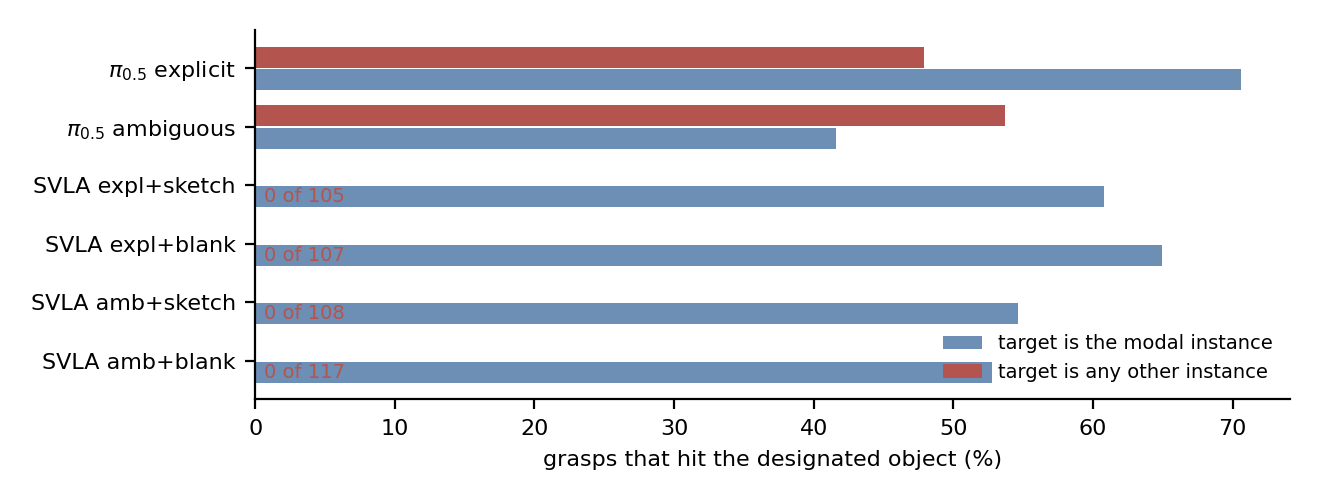
\includegraphics[width=0.64\textwidth]{figures/fig_selection.png}
\end{center}
\vspace{-8pt}
{\footnotesize \textbf{Figure 1.} Of the grasps an arm actually completes, the
share that landed on the designated object. Split by whether that object is the
modal instance. The four fine-tuned arms have no red bar because the count is
zero, not missing.}

Across the four arms, on scenes whose target is not the modal instance, the
policy grasped something \numOtherGrasps{} times and hit the designated object
\textbf{\numOtherHits{}} times. In those same scenes it reached for the modal
instance on \numModalPullExpl\% of its grasps. $\pi_{0.5}$ hits the target
\numBaselineOtherHits\% of the time there.

Indifference to the conditioning predicts roughly chance --- around 30\% with
two to five candidate bowls in frame. Zero out of \numOtherGrasps{} is far below
chance, and a policy cannot land below chance by ignoring its inputs. It lands
there by reaching a fixed position: right when the target happens to sit there,
never when it does not.

\heading{Table 2 --- grasped the designated object, by tier}
\begin{center}\small
\begin{tabular}{lrrrrr}
\toprule
Tier & $n$ & SVLA expl+sketch & SVLA amb+blank & $\pi_{0.5}$ expl & $\pi_{0.5}$ amb \\
\midrule
\tabTiers
\bottomrule
\end{tabular}
\end{center}
\vspace{-2pt}
{\footnotesize Tier is a property of the scene: \texttt{control} one-to-one,
\texttt{referential} many-to-one, \texttt{directional} one-to-many,
\texttt{both} many-to-many. $n$ is rollouts per tier in one arm.}

\begin{center}
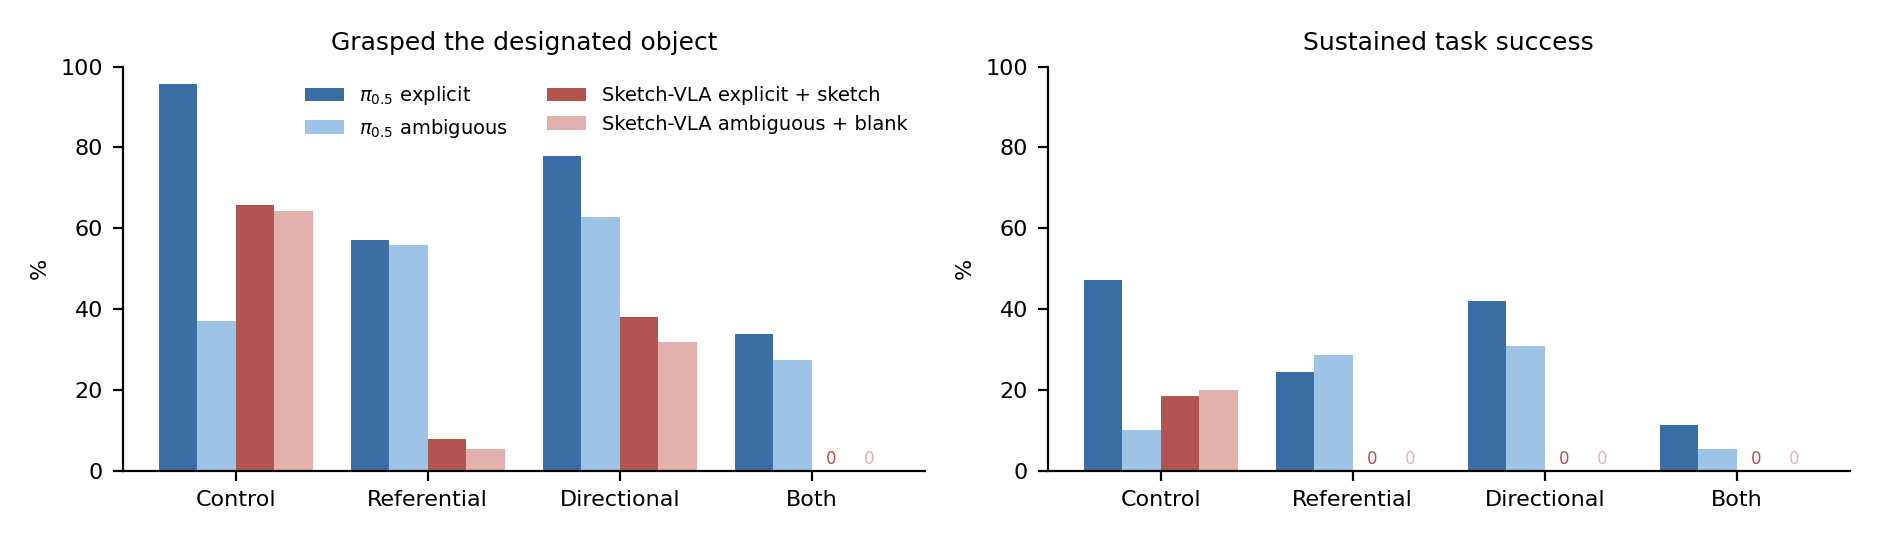
\includegraphics[width=0.78\textwidth]{figures/fig_tier_breakdown.png}
\end{center}
\vspace{-8pt}
{\footnotesize \textbf{Figure 2.} The same split across tiers. The fine-tuned
checkpoint is competitive only on \texttt{control}, where one candidate object
makes selection unnecessary, and collapses everywhere selection is required.
Zeros are printed rather than left as absent bars.}

\heading{What I ruled out before concluding this}
\begin{itemize}
  \item \textbf{Referent labelling.} The sketch referent derived at eval time
    matches the manifest ground truth 38/38, object and destination both. The
    zero is not a mislabelled target.
  \item \textbf{Image orientation.} The eval feeds unrotated frames on purpose:
    \texttt{sketch\_libero} was rendered in the simulator's own orientation,
    which is the orientation the sketches were authored in. I dump the first
    model-input frame of every scene and the circle lands on the intended bowl.
  \item \textbf{Sketch delivery.} A smoke gate refuses an empty sketch in
    \texttt{real} mode and a non-empty one in \texttt{blank} mode, and the mode
    is stamped into every row, so ``blank on purpose'' and ``blank because the
    lookup missed'' cannot be confused.
  \item \textbf{Budget parity.} Both models ran 240 steps and 48 inference calls
    per rollout, replanning every 5. Identical in every row of both runs.
  \item \textbf{Training prompts.} \texttt{prompt\_from\_task=True} is set for
    this variant, so the caption did reach the model during fine-tuning. The
    insensitivity is not a missing input.
\end{itemize}

\heading{Limitation}
The contrasts above are unpaired. \texttt{init\_state\_hash} is identical across
all four arms (\numPairInit\% of rows), but \texttt{init\_warmstart\_hash}
agrees on only \numPairWarm\% --- rollout 0 of each scene. The scene environment
is opened once and reused for all 14 rollouts, and \texttt{set\_init\_state()}
restores \texttt{qpos}/\texttt{qvel} without clearing MuJoCo's
\texttt{qacc\_warmstart}, which therefore carries over from the previous
rollout. With 532 rollouts per arm the unpaired test has ample power and the
paired subset agrees, so I do not believe this changes the answer --- but it
should be fixed before the next run, by zeroing \texttt{qacc\_warmstart} and
\texttt{act} after the reset.

\heading{What I recommend}
I would not spend GPU time on the object and goal transfer suites. The
checkpoint fails in-distribution, so a transfer number would carry no
information.

The likely cause sits in the fine-tuning configuration rather than in the idea:
\texttt{batch\_size} is 2, so 30{,}000 steps see 60{,}000 samples; warmup covers
a third of the run; and \texttt{decay\_steps} is $10^{6}$ against a
30{,}000-step run, so the learning rate never decays. Before paying for another
full run I would add a gate at every checkpoint save --- one scene, two captions
naming different bowls, compare the predicted action chunks. If they agree
within noise the run is already dead and can be stopped in minutes.

\end{document}
